\chapter{\acs{ros2} Interface for Physical E-puck2}
\label{chap:physical}
\shorttitle{\nameref{chap:physical}}

Details about \ac{ros2} interface implementation on e-puck2 physical robot will be given in this chapter.
Even though the objective is to create the same \ac{ros2} interface as one explained in the previous chapter the implementation is very different.
The difference mostly comes from the physical interface to the sensors and actuators, performance limitations, and \ac{cpu} architecture.
Therefore, these differences will be emphasized in this chapter.

\section{Introduction}

Pi-puck extension uses \ac{i2c} and \ac{usb} to communicate with sensors and actuators available on the e-puck2 robot (see Fig. \ref{fig:physical:general}).

\begin{figure}[H]
    \centering
    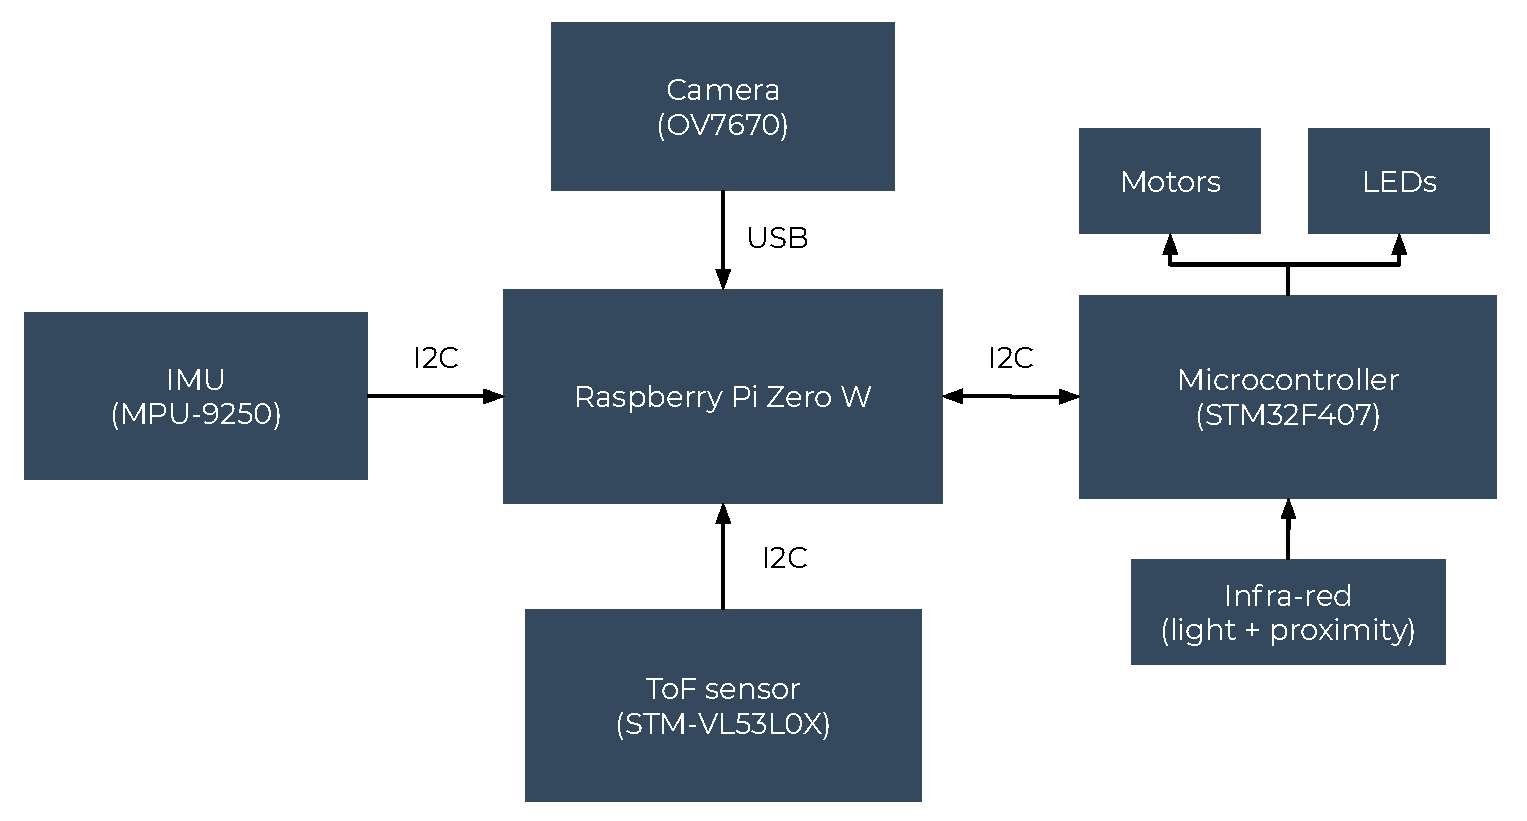
\includegraphics[width=\textwidth]{physical/figures/general.pdf}
    \caption{Components utilized in \ac{ros2} driver}
    \label{fig:physical:general}
\end{figure}

In case \acp{led}, motors, and infrared sensors the communication is done through on-board \ac{mcu}.
In the case of infrared sensors, this is necessary as Raspberry Pi Zero W doesn't have any \ac{dac} module. 
Therefore, the \ac{mcu} acts as a slave that stands between analog sensors and actuators, or actuators that require deterministic updates (motors).
With \ac{imu} and the \ac{tof} sensor, Raspberry Pi Zero Zero W communicates directly over \ac{i2c}, while with the camera the communication is done over \ac{usb}. 

\begin{table}[H]
    \centering
    \begin{tabular}{|l|l|}
        \hline
        \textbf{Sensor function} & \textbf{Sensor model} \\
        \hline
        Camera & Omnivision OV7670 CMOS\footnote{Datasheet of the OV7670 sensor is available at \url{http://projects.gctronic.com/epuck2/doc/OV7670.pdf}} \\
        \hline
        Distance and light sensors & TCRT1000 \\
        \hline
        \ac{imu} & InvenSense MPU-9250 \\
        \hline
        \ac{tof} & STM-VL53L0X \cite{lakovic_application_2019} \\
        \hline
    \end{tabular}
    \caption{List of the relevant sensors available on e-puck2 robot shown in Fig. \ref{fig:physical:general}}
    \label{tab:physical:sensors}
\end{table}

The protocol used to communicate with the sensors is explained in the corresponding sensor's documentation, while the communication with the \ac{mcu} is specified by the format shown in Table \ref{tab:physical:rpi_to_mcu} and Table \ref{tab:physical:mcu_to_rpi}.

\begin{table}[H]
    \centering
    \begin{tabular}{c|c|c|c}
    \hline
    \textbf{Left speed (2)} & Right speed (2) & Speaker (1) & LED[1,3,5,7] (1)  \\
    \hline
    LED2 (3) & LED4 (3) & LED6 (3) & LED8 (3) \\
    \hline
    Settings (1) & \textbf{Checksum (1)} & & \\
    \hline
    \end{tabular}
    \caption[Message format sent from the Raspberry Pi Zero W to the \ac{mcu}]{Message format sent from the Raspberry Pi Zero W to the \ac{mcu}. Bolded fields highlight the most and the least significant bytes in the packet.}
    \label{tab:physical:rpi_to_mcu}
\end{table}

\begin{table}[H]
    \centering
    \begin{tabular}{c|c|c|c}
    \hline
    \textbf{8 x Prox (16)} & 8 x Ambient (16) & 4 x Mic (8) & Selector + button (1) \\
    \hline
    Left steps (2) & Right steps (2) & TV remote (1) & \textbf{Checksum} \\
    \hline
    \end{tabular}
    \caption[Message format sent from the \ac{mcu} to the Raspberry Pi Zero W]{Message format sent from the \ac{mcu} to the Raspberry Pi Zero W. Bolded fields highlight the most and the least significant bytes in the packet.}
    \label{tab:physical:mcu_to_rpi}
\end{table}

\section{\ac{ros2} on Raspberry Pi OS}
Before \ac{ros2} driver is created \ac{ros2} has to be installed on the Raspberry Pi Zero W.
The board comes with \ac{cpu} with arm32 architecture and Raspberry Pi OS.
This configuration is not officially supported by \ac{ros2} and standard installation procedure using \acs{os}' package manager doesn't work.
The closest official support is a source compilation for Debian Buster placed as a tier 3 support\footnote{\ac{ros2} supported platforms are defined by REP 2000 available at \url{https://www.ros.org/reps/rep-2000.html\#foxy-fitzroy-may-2020-may-2023}}.
This means that \ac{ros2} has to be cross-compiled and that potential incompatibilities have to be manually resolved.

Since the \ac{ros2} driver is intended for a wide range of users the installation procedure has to be user-friendly.
In that purpose, three user guides are created to simplify the installation procedure, using pre-configured \ac{sdcard}, compilation on Raspberry Pi Zero W, and cross-compilation from the user's \ac{pc}.
A comparison of these methods is given by Table \ref{tab:physical:installation}.

\begin{table}[H]
    \begin{adjustwidth}{-1.5in}{-1.5in}
    \centering
    \begin{tabular}{|l|c|c|c|}
        \hline
        & \textbf{Using image} & \textbf{Compilation on the board} & \textbf{Cross-compilation} \\
        \hline
        Compilation speed & ++ & - & + \\
        \hline
        Easy to use & ++ & - & -- \\
        \hline
        Flexibility & -- & ++ & + \\
        \hline
    \end{tabular}
    \caption{Comparison of different installation methods provided in the scope of the project}
    \label{tab:physical:installation}
    \end{adjustwidth}
\end{table}

Using the existing image with \ac{ros2} and other tools configured is the easiest approach for the users.
The problem appears once the user has to upgrade the \ac{ros2} version, install a new package, or to develop a custom package that has a lot of dependencies as compilation time is slow.
For those use cases, cross-compilation tools are provided.

\subsection{\ac{ros2} Cross-compilation}
In the scope of the project, tools are built to help with the process of \ac{ros2} cross-compilation.
All cross-compilation dependencies and configurations are packaged into a Docker container\footnote{Thorough guide about the \ac{ros2} cross-compilation is available at \url{https://github.com/cyberbotics/epuck_ros2/tree/master/installation/cross_compile}}.
This means that the user doesn't need to worry about host \ac{os} and tools compatibility. 

\begin{figure}[H]
    \centering
    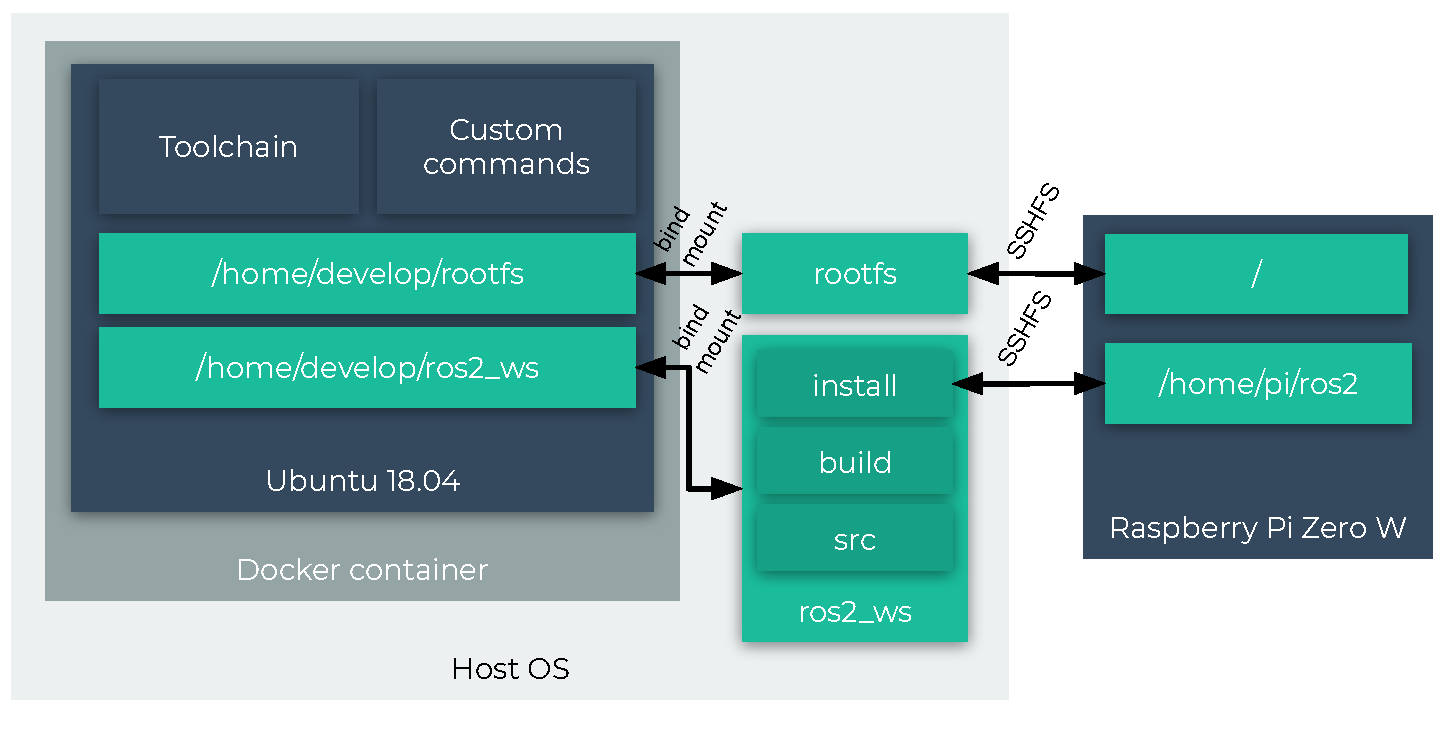
\includegraphics[width=\textwidth]{physical/figures/cross_compilation.pdf}
    \caption{\ac{ros2} cross-compilation setup}
    \label{fig:physical:cross_compilation}
\end{figure}

The typical setup of using the cross-compilation tools built within this project is shown in Fig. \ref{fig:physical:cross_compilation}.
Boxes in green represent directories while the others are software tools.
\texttt{ros2\_ws} is \ac{ros2} workspace, it contains source files, temporary build files and compiled output, libraries and executable.
The source code available in this directory is compiled with cross-compilation tools in the Docker container while the result stays available on the host \ac{os}.
To build certain packages, compilers need filesystem of the Raspberry Pi Zero W (\texttt{rootfs}) to compile and link dependencies available on the board.
Both directories are available in the Docker container as well as on the host \ac{os}.

Once the \ac{ros2} packages are compiled they can be used by copying \texttt{ros\_ws/install} directory or by mounting it to the Raspberry Pi Zero W.
Although, mounting the directory can significantly increase the productivity as the process of copying the files can be avoided.

% TODO: Typical errors

\section{Programming Language}
Initially, \ac{ros2} driver, with a few basic features, for the physical e-puck2 is implemented in Python programming language.
However, as the \ac{ros2} driver included more sensors the \ac{cpu} load was too high to handle other functionalities. 

\begin{figure}[H]
\centering
\begin{subfigure}{.8\textwidth}
  \centering
  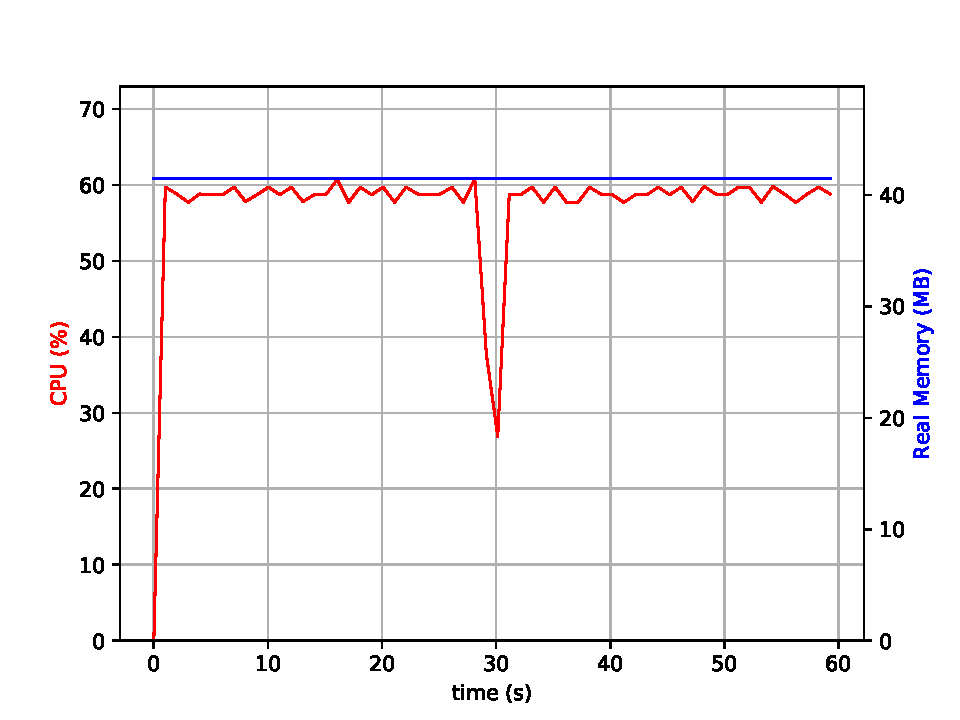
\includegraphics[width=\linewidth]{physical/figures/rpi_py_32ms}
  \caption{\ac{cpu} and \ac{ram} load with Python}
  \label{fig:physical:py_vs_cpp:py}
\end{subfigure}
\begin{subfigure}{.8\textwidth}
  \centering
  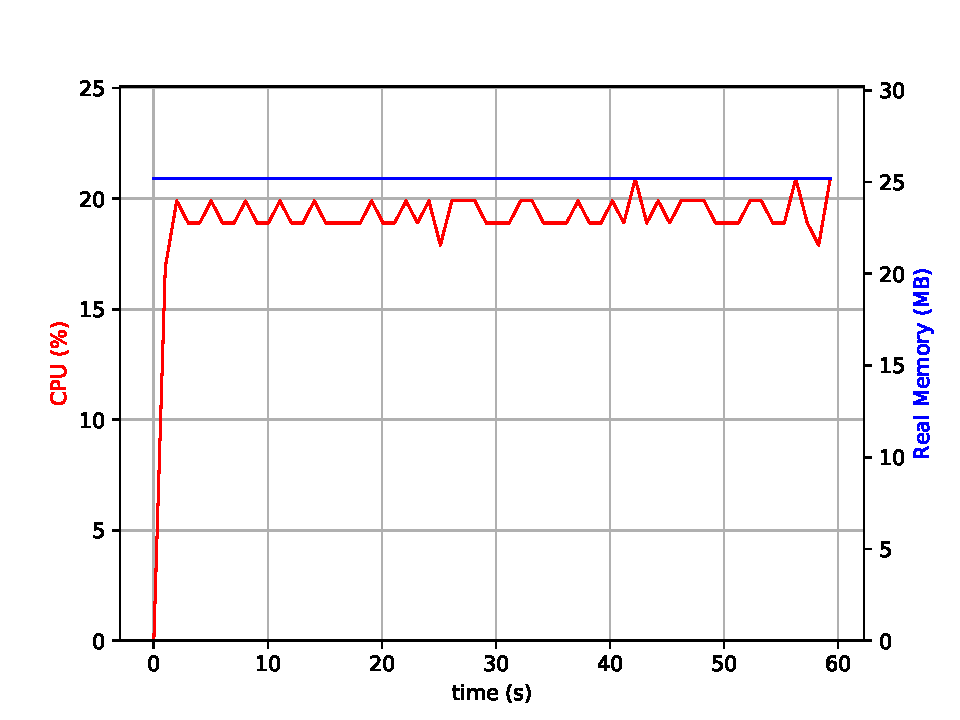
\includegraphics[width=\linewidth]{physical/figures/rpi_cpp_32ms}
  \caption{\ac{cpu} and \ac{ram} load with C++}
  \label{fig:physical:py_vs_cpp:cpp}
\end{subfigure}
\caption[Performance comparison of implementations in Python and C++]{Performance comparison of the similar node \ac{ros2} node implemented in Python and C++. The \ac{cpu} and \ac{ram} load is measured using \texttt{psrecord} tool}
\label{fig:physical:py_vs_cpp}
\end{figure}

In Fig. \ref{fig:physical:py_vs_cpp} performances of Python and C++ implementation of similarly implemented \ac{ros2} node that provide the same functionalities are given.
More precisely, they both publish odometry data, measurements from eight distance sensors, laser scan, and they are both subscribed to the velocity control topic.
In the figure, we can observe that \ac{cpu} usage is three times lower while \ac{ram} is almost two times lower.
This analysis in early stage of implementation steered the development towards C++\footnote{One of the bottlenecks was in \ac{ros2} client library for Python (\texttt{rclpy}) related to timer implementation - \url{https://github.com/ros2/rclpy/issues/520}. Fixing it improved the performances, but C++ implementation was still more efficient.}.

% The exact command to measure the load is \texttt{psrecord \$(pgrep epuck2\_driver) --interval 1 --plot plot.pdf --duration 60}

\section{Camera}
As mentioned before, the camera available on e-puck2 (Omnivision OV7670 CMOS) captures images at 15 \acs{fps} in resolution of 640x480.
Compared to the simulation, data produced by the camera has to be efficiently processed and intrinsic camera parameters have to be determined.

\subsection{Camera Optimization}
Our preliminary investigation showed that the \ac{ros2} driver wasn't able to publish images more frequently than 3-4 \acs{fps} (thorough analysis is available in Chapter \ref{chap:results}).
Publishing raw (uncompressed) images would cause the network to become a bottleneck while compressing the images before transmitting would put a high \ac{cpu} load, effectively limiting \ac{fps}.
Fortunately, there is \ac{gpu} available on Raspberry Pi Zero W on which certain image manipulation tasks can be offloaded.

\subsubsection{Introduction}
A brief overview on \ac{gpu} on Raspberry Pi Zero W will be given first. Typical architecture of the \ac{gpu} and the related components is given by the following figure (Fig. \ref{fig:physical:gpu_architecture}):
 
 \begin{figure}[H]
    \centering
    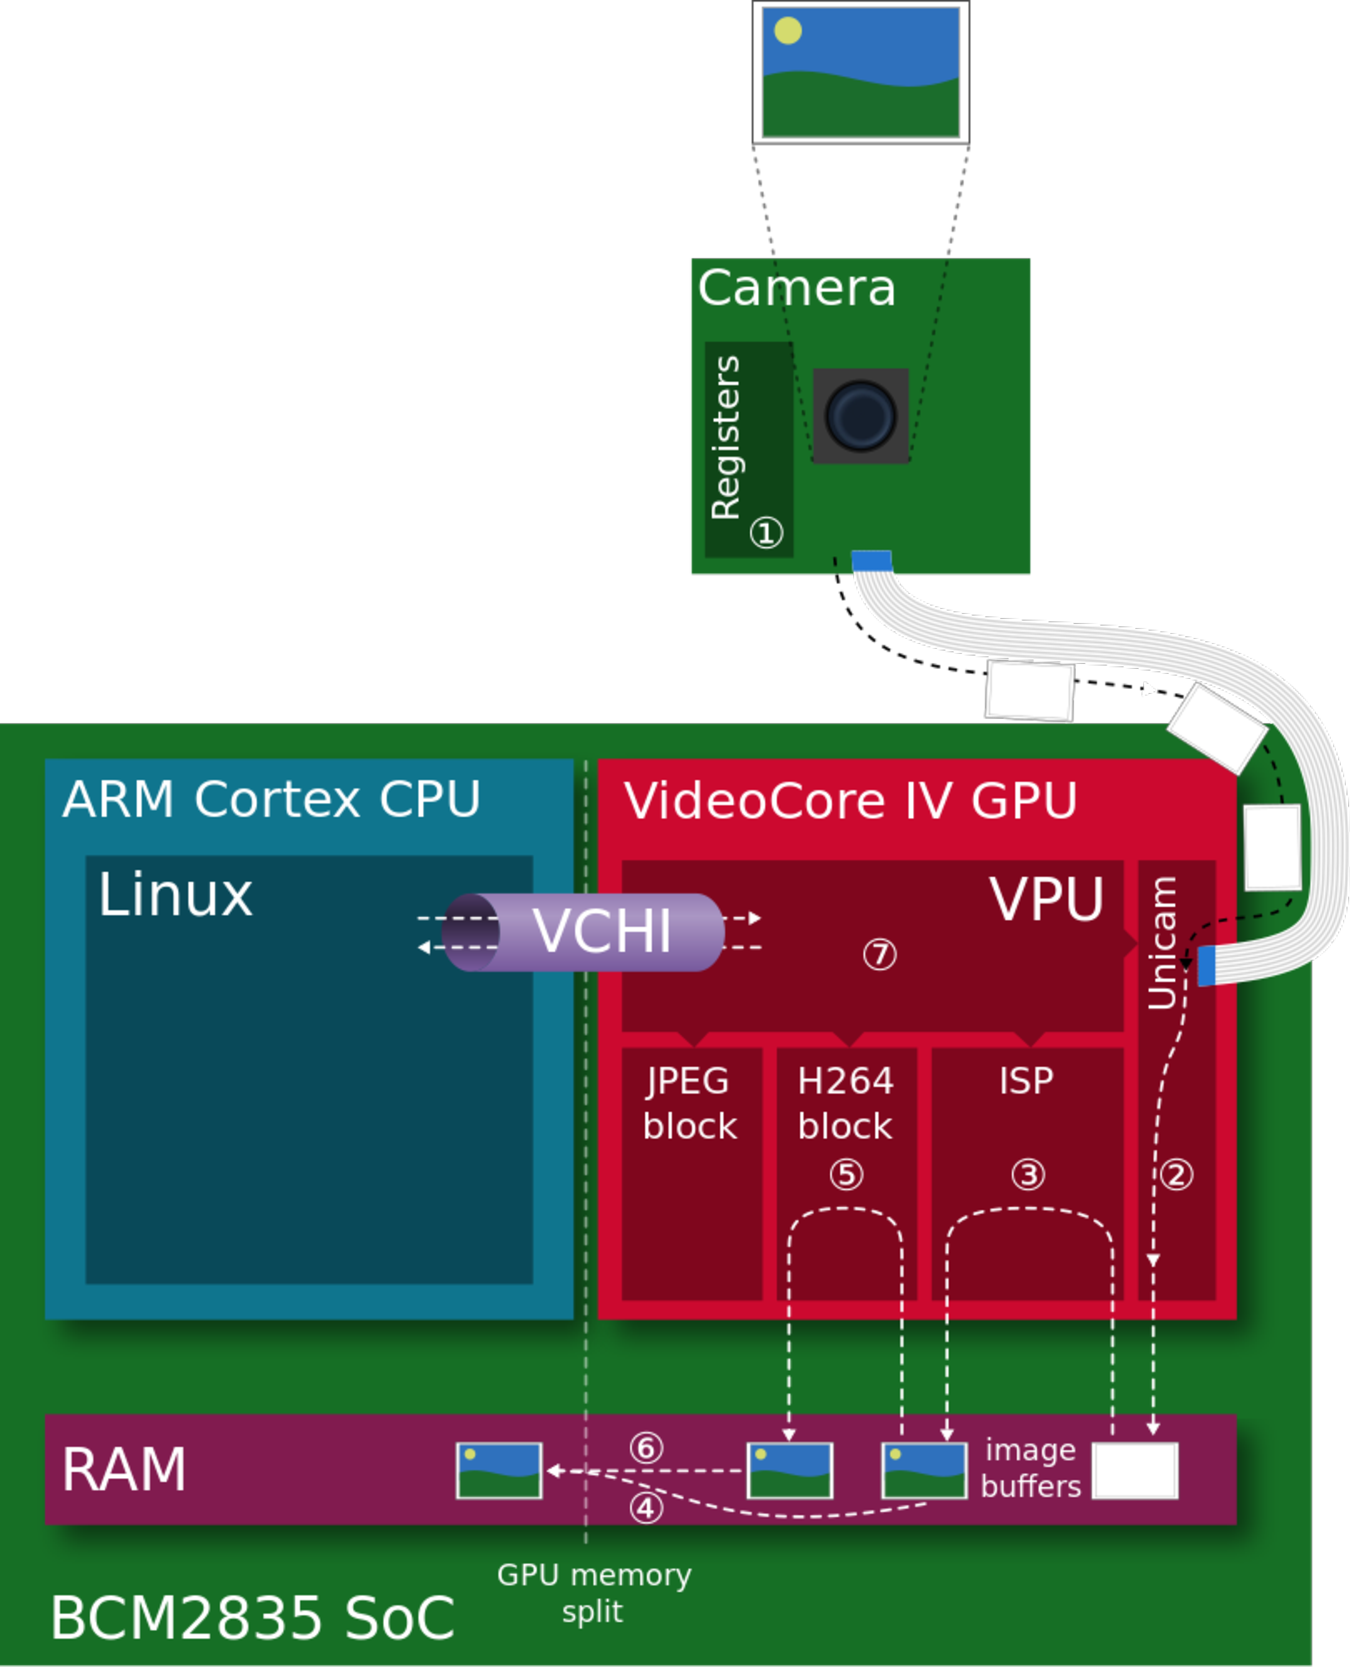
\includegraphics[width=0.8\textwidth]{physical/figures/gpu_architecture}
    \caption{\ac{gpu} architecture \cite{noauthor_videocore_nodate-1}}
    \label{fig:physical:gpu_architecture}
\end{figure}

In the figure, there are three main components on the \ac{soc}, \ac{cpu}, \ac{gpu} and \ac{ram}.
Further, \ac{gpu} has it's own computational components dedicated for different image processing tasks.
These components are orchestrated by \ac{vcos} (abstraction layer on top of an \ac{rtos}) which also reads images from the camera.
Signaling between \ac{cpu} and \ac{gpu} is done through \ac{vchi} while the images are shared by storing them on \ac{ram}.
From the software point of view, \ac{mmal} library is used to interact with the \ac{gpu}.
The library is based on \ac{omx} and the goal is to ensure consistent interface across all \acp{gpu} available in different models of Raspberry Pi.
For comprehensive explanation about hardware blocks read \cite{noauthor_videocore_nodate-1} and for software \cite{noauthor_videocore_nodate}, both are great sources of information.

\subsubsection{\ac{ros2} Camera Driver Implementation}
There are a few available \ac{ros}1 and \ac{ros2} packages that implement \ac{gpu} accelerated image acquisition and processing.
Unfortunately, these packages expect the camera to be connected via \ac{csi} which is not the case in e-puck2. 
Therefore, the whole \ac{ros2} camera node is implemented from scratch, including image acquisition based on \ac{v4l2} and image processing (compression and resizing) based on \ac{mmal}.
 
 \begin{figure}[H]
    \centering
    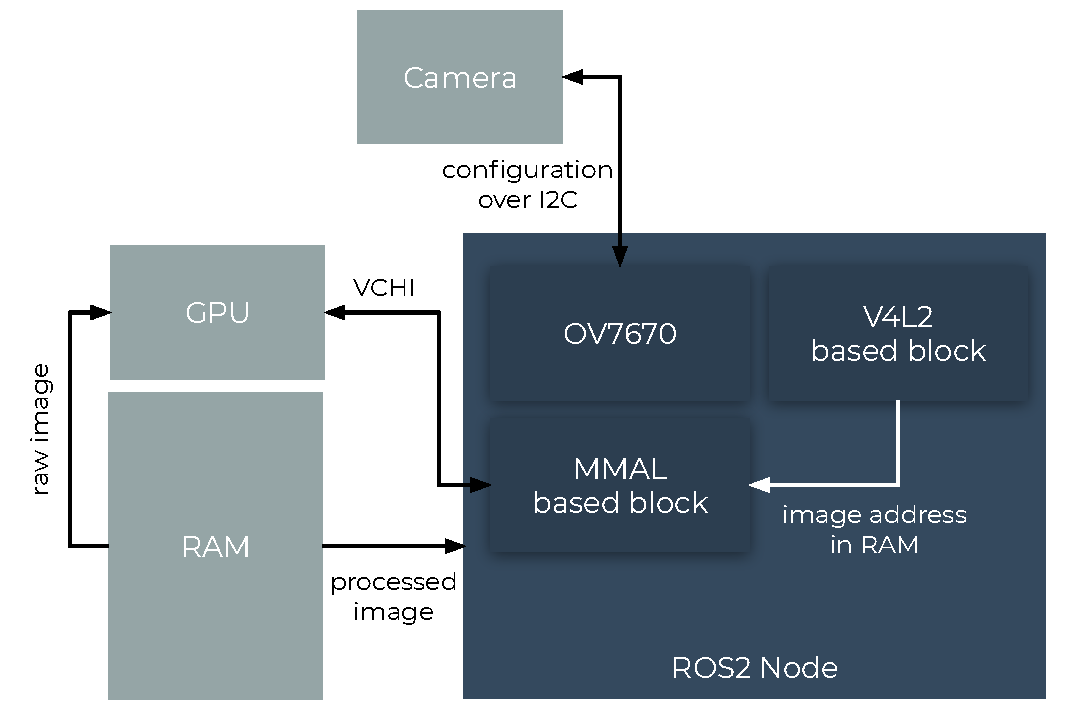
\includegraphics[width=0.8\textwidth]{physical/figures/camera_software_architecture.pdf}
    \caption{Camera software architecture}
    \label{fig:physical:camera_software_architecture}
\end{figure}
 
 In Fig. \ref{fig:physical:camera_software_architecture} a software architecture of the camera node is given. 
 Initially, the camera is configured over \ac{i2c} (block \texttt{OV7670}) and then \ac{v4l2} is used to initiate image capture and store it to the \ac{ram}.
 The pointer to the image is passed through \ac{mmal} block which interacts with \ac{gpu} to compress and resize it. 
 Finally, \ac{gpu} stores the processed image to the \ac{ram} and the pointer the processed image is available to the \ac{ros2} camera node.
 The node packs it into the corresponding messages type and publishes it.
 
 \subsubsection{\ac{ros2} Camera Driver Usage}
 Since the camera transmits the images through the network compressed they have to be uncompressed once the target computer is reached.
 
\begin{figure}[H]
    \centering
    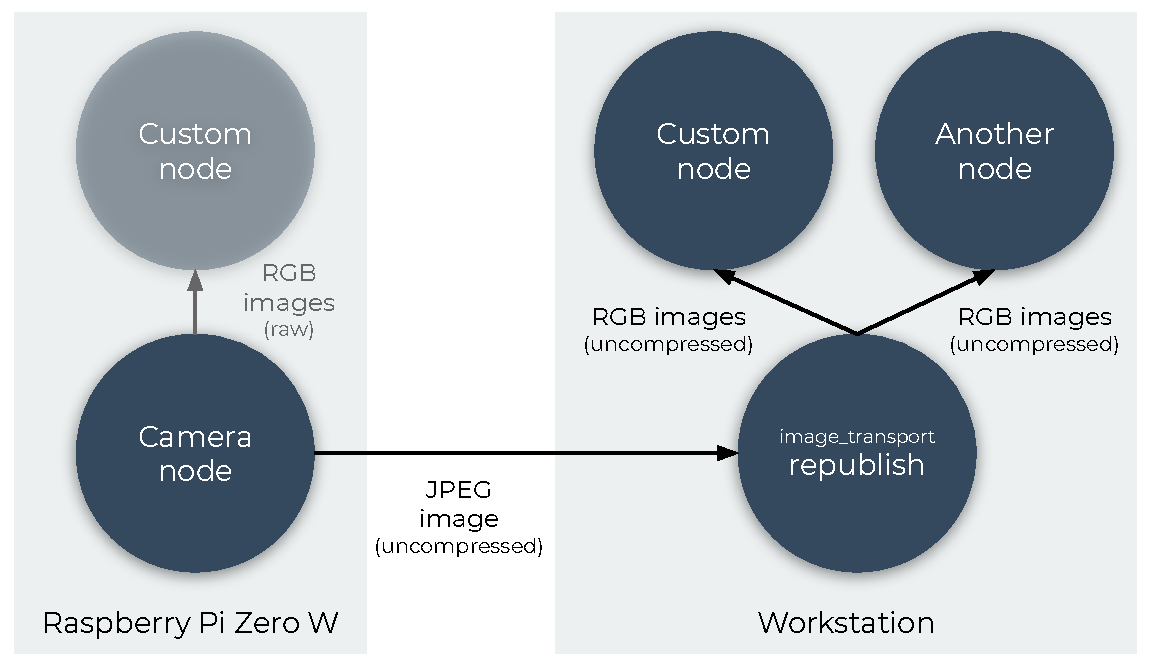
\includegraphics[width=0.8\textwidth]{physical/figures/camera_ros_images.pdf}
    \caption{Image flow within \ac{ros2} application}
    \label{fig:physical:camera_ros_images}
\end{figure}

Fig. \ref{fig:physical:camera_ros_images} shows typical flow of images within \ac{ros2} application.
The camera node will publish \acs{rgb} or \acs{jpeg} compressed images depending on which topic a user is subscribed to.
From the user's perspective \ac{rgb} images desired as pixel-wise operations can be done directly, without decompression.
Therefore, if a user has a custom node running on the Raspberry Pi Zero W the user should subscribe to \ac{rgb} images.
Otherwise, if the user wants to use on the workstation the user should run \texttt{image\_transport/republish} node besides.
The node decompresses the images on the workstation and publishes \ac{rgb} to all local nodes.
This way, a custom node by the user will not change and the only additional action that the user has to do if working on the workstation is running \texttt{image\_transport/republish} node.
 
\subsubsection{Camera Calibration}
In comparison with \ac{ros2} node for the simulated robot intrinsic parameters of the Omnivision OV7670 camera are not known.
These parameters can be found through a calibration process. The process consists of capturing many images, which is known as the physical position of points, and then performing non-linear optimization to find parameters that project these points from the 3D world to 2D plane \cite{lukic_dual_nodate}. This process is automated by creating a custom \ac{ros2} node that relies on OpenCV's calibration module.

\subsection{Differential Drive}
Besides the performance limitations of the Raspberry Pi Zero W that cause issues, there are other limitations as well. In the case of odometry, in Table \ref{tab:physical:rpi_to_mcu}, you can notice that number of ticks for left and the right wheel is limited to 2 bytes. Taking into account it is a signed number (can take a value from -32767 to 32767) and that there are 1000 ticks per revolution it can make around 32 revolutions before overflow (or $ 2 \pi R \frac{32767}{1000} = 4.11m $). This means that the robot's odometry will become completely wrong after around 4 meters. To avoid this, the following simple approach is applied:

\vspace*{.4cm}
\begin{algorithm}[H]
\SetKwInOut{Input}{input}
\SetKwInOut{Output}{output}
\Input{%
    $\bm{N_{overflow}}$ -- Number of overflows (it can be negative) \newline 
    $\bm{N_{grace}}$ -- Constant which represents the maximum difference in number of ticks between two sequential samples \newline 
    $\bm{P_{ticks}}$ -- Number of ticks in the previous sample \newline 
    $\bm{C_{ticks}}$ -- Number of ticks received from the sensor
}
\Output{%
    $\bm{T_{ticks}}$ -- Total (corrected) number of ticks
}

\If{$ |P_{ticks} - C_{ticks}|> 2^{15} - N_{grace} $}{
    \eIf{$P_{ticks} > 0 \land C_{ticks} < 0$}{
        increment $N_{overflow}$\;
    }{
        decrement $N_{overflow}$\;
    }
}
$ T_{ticks} \leftarrow 2^{16} N_{overflow} + C_{ticks} $\;

\caption{Overflow protection algorithm}
\label{alg:physical:overflow}
\end{algorithm}
\vspace*{.4cm}

By applying Alg. \ref{alg:physical:overflow}, in $ T_{ticks} $ a total number of ticks will be stored, taking overflows into the consideration. It is important set $ N_{grace} $ reasonably big such that $ |P_{ticks} - C_{ticks}| > N_{grace} $ is only satisfied when the overflow occurs.

\section{Software Quality Assurance}
As a part of ROSIN\footnote{Software Quality Assurance propositions of ROSIN project can be fount at \url{https://www.rosin-project.eu/software-quality-assurance}}, this master project has to incorporate software engineering best practices such as continuous integration \cite{meyer_continuous_2014}, unit testing and code reviews. Those practices are fully utilized throughout the whole project and they will be briefly explained here.

\subsection{\ac{ros2} Node Unit Tests}

The unit tests are implemented according to the standard procedure recommended by \ac{ros2}. Two \ac{ros2} nodes are executed, one node is the actual node we want to test while the other one simulates the rest of the application and executes tests. 

\begin{figure}[H]
    \centering
    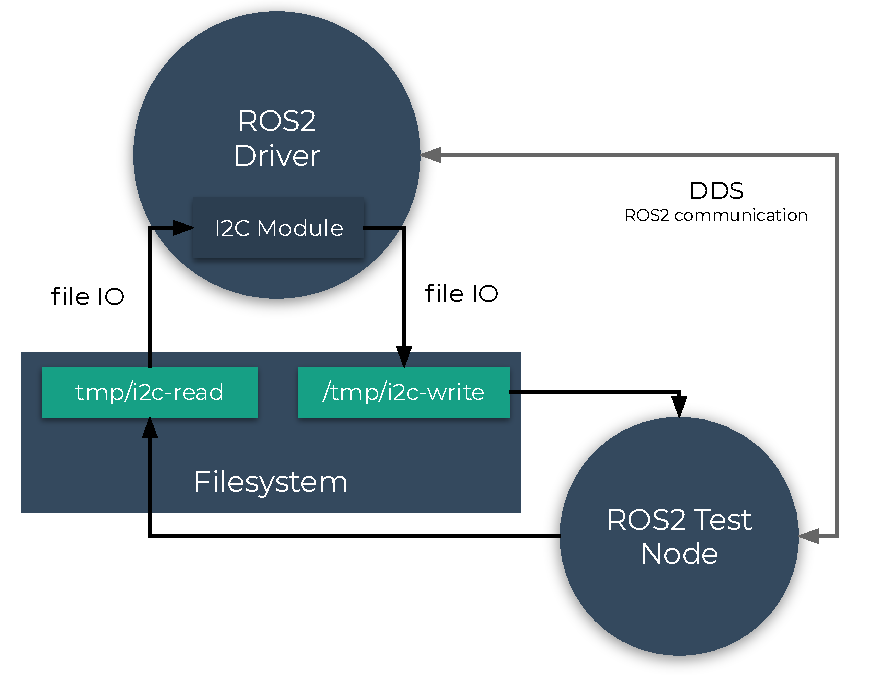
\includegraphics[width=0.8\textwidth]{physical/figures/mocking.pdf}
    \caption{Testing communication with the microcontroller}
    \label{fig:physical:mocking}
\end{figure}

A concrete example for testing of the \ac{ros2} driver is given in Fig. \ref{fig:physical:mocking}. In the figure, \ac{ros2} test node is used to emulate the rest of the \ac{ros2} application. For example, it can publish a message to \texttt{/cmd\_vel} and set angular velocity.
The \ac{ros2} driver should receive the message and send corresponding motor velocity through \ac{i2c}. To verify whether proper commands are sent over \ac{i2c} a special \ac{i2c} module is created.
It implements two modes, in regular mode it interacts with \ac{i2c} directly while in testing, it writes everything to the filesystem. 
This way, \ac{ros2} test node has an opportunity to test commands addressed to the \ac{i2c}.

All unit tests are based on Python's standard unit testing framework \texttt{unittest} and \ac{ros}' \texttt{launch\_test}.

\subsection{Code Quality Tests}
Besides the unit tests, many tests for static code analysis are used as well.
The following tests are used to perform code quality analysis:
\begin{itemize}
    \item \texttt{cppcheck} detects undefined behavior (e.g. dead pointers, division by zero or integer overflows) and security issues (e.g. buffer errors and information leaks) in C++ code.
    \item \texttt{cpplint} verifies whether the user follows C++ best practices and it detects syntax errors.
    \item \texttt{clang\_format} recommends how the C++ code should be formatted and it fails if the code is not formatted properly. 
    \item \texttt{lint\_cmake} verifies whether CMake files follow the best practices.
    \item \texttt{flake8} enforces Python code to follow a style guide.
    \item \texttt{pep257} verifies if docstrings in Python code are properly formatted.
    \item \texttt{xmllint} verifies whether XML files follow the best practices.
    \item \texttt{copyright} check if the copyright header is present in the files.
\end{itemize}

All tests are performed on almost all files available in the source code. 

\subsection{\acl{ci}}
Unit tests, code quality tests, and more are executed in the scope of \ac{ci}.
It means that the source code is stored in Git repository and that series of tests are executed every time a new change is pushed.
In particular, every time a new commit is pushed a Docker container is created, \ac{ros2} environment is created, static code analysis is done, the package is built and the packages are unit tested.
If any of these actions fail the whole test is considered a failure and a developer is forced to fix the error.
